\documentclass[12pt,fleqn]{article}\usepackage{../../common}
\begin{document}
Özellik İşlemek (Feature Engineering)

Veri madenciliğinde "veriden veri yaratma" tekniği çok kullanılıyor; mesela
bir sipariş veri satırında o siparişin hangi zamanda (timestamp) olduğunu
belirten bir kolon varsa (ki çoğu zaman vardır), bu kolonu "parçalayarak"
ek, daha genel, özetsel bilgi kolonları yaratılabilir. Ya da kategoriksel
verileri pek çok farklı şekilde sayısal hale çevirebiliriz, mesela 1-hot
kodlama ile N kategori N kolon haline gelir, eldeki kategoriye tekabül eden
öğe 1 diğerleri sıfır yapılır. 

Özellik işlemenin önemi yapay öğrenme açısından önemi var, mesela bir SVM
sınıflayıcısını en basit haliyle siyah/beyaz görüntüden sayı tanıma
probleminde kullandık, ve diyelim yüzde 70 başarı elde ettik. Şimdi çok
basit bir yeni özellik yaratalım, görüntüyü dikey ikiye bölelim, ve üstteki
ve alttaki siyah noktaları toplayarak iki yeni kolon olarak görüntü
matrisine ekleyelim. Bu yeni özellikleri kullanınca basit sınıflayıcının
yüzde 20 kadar tanıma başarısında ilerleme kaydettiğini göreceğiz!

Not: Derin yapay sınır ağları teknikleri ile özellik işlemeye artık gerek
olmadığı söylenir, bu büyük ölçüde doğru. Bir DYSA farklı seviyelerdeki pek
çok farklı nöronları üzerinden aslında üstte tarif edilen türden yeni
özellikleri otomatik olarak yaratır, ögrenir. Fakat yine de yeni
özellikleri elle yaratma tekniklerini bilmek iyi.

Şimdi farklı yöntemlere bakalım.

Zaman Kolonlarını Zenginleştirmek

Zaman kolonları çoğu zaman saniyeye kadar kaydedilir, bu bilgiyi alıp
mesela ay, mevsim, haftanın günü, saat, iş saati mi (9-5 arası), akşam mı,
sabah mı, öğlen mi, vs. gibi ek bilgiler çıkartılabilir. Tüm kolonlar veri
madenciliği algoritmasına verilir, ve algoritma belki öğlen saati ile
sipariş verilmiş olması arasında genel bir bağlantı bulacaktır.

Python + Pandas ile bir zaman kolonu şöyle parçalanabilir, örnek veri
üzerinde görelim, sadece iki kolon var, müşteri no, ve sipariş zamanı,

\begin{minted}[fontsize=\footnotesize]{python}
import pandas as pd
from StringIO import StringIO
s = """customer_id;order_date
  299;2012-07-20 19:44:55.661000+01:00
  421;2012-02-17 21:54:15.013000+01:00
  437;2012-02-20 22:18:12.021000+01:00
  463;2012-02-20 23:46:21.587000+01:00
  482;2012-05-21 09:50:02.739000+01:00
  607;2012-02-21 11:57:12.462000+01:00
  641;2012-02-21 13:40:28.088000+01:00
  674;2012-08-21 14:53:15.851000+01:00
  780;2012-02-23 10:31:05.571000+01:00
  """
df = pd.read_csv(StringIO(s),sep=';', parse_dates=True)

def f(x):
  tmp = pd.to_datetime(x['order_date'])
  tpl = tmp.timetuple(); yymm = int(tmp.strftime('%m%d'))
  spring = int(yymm >= 321 and yymm < 621)
  summer = int(yymm >= 621 and yymm < 921)
  fall = int(yymm >= 921 and yymm < 1221)
  winter = int( spring==0 and summer==0 and fall==0 )
  warm_season = float(tpl.tm_mon >= 4 and tpl.tm_mon <= 9)
  work_hours = float(tpl.tm_hour > 9 and tpl.tm_hour < 17)
  morning = float(tpl.tm_hour >= 7 and tpl.tm_hour <= 11)
  noon = float(tpl.tm_hour >= 12 and tpl.tm_hour <= 14)
  afternoon = float(tpl.tm_hour >= 15 and tpl.tm_hour <= 19)
  night = int (morning==0 and noon==0 and afternoon==0)

  return pd.Series([tpl.tm_hour, tpl.tm_mon,
                    tpl.tm_wday, warm_season,
                    work_hours, morning, noon, afternoon, night,
                    spring, summer, fall, winter])

cols = ['ts_hour','ts_mon','ts_wday','ts_warm_season',\
  'ts_work_hours','ts_morning','ts_noon','ts_afternoon',\
  'ts_night', 'ts_spring', 'ts_summer', 'ts_fall', 'ts_winter']

df[cols] = df.apply(f, axis=1)
print df[cols]
\end{minted}

\begin{verbatim}
   ts_hour  ts_mon  ts_wday  ts_warm_season  ts_work_hours  ts_morning  \
0     18.0     7.0      4.0             1.0            0.0         0.0   
1     20.0     2.0      4.0             0.0            0.0         0.0   
2     21.0     2.0      0.0             0.0            0.0         0.0   
3     22.0     2.0      0.0             0.0            0.0         0.0   
4      8.0     5.0      0.0             1.0            0.0         1.0   
5     10.0     2.0      1.0             0.0            1.0         1.0   
6     12.0     2.0      1.0             0.0            1.0         0.0   
7     13.0     8.0      1.0             1.0            1.0         0.0   
8      9.0     2.0      3.0             0.0            0.0         1.0   

   ts_noon  ts_afternoon  ts_night  ts_spring  ts_summer  ts_fall  ts_winter  
0      0.0           1.0       0.0        0.0        1.0      0.0        0.0  
1      0.0           0.0       1.0        0.0        0.0      0.0        1.0  
2      0.0           0.0       1.0        0.0        0.0      0.0        1.0  
3      0.0           0.0       1.0        0.0        0.0      0.0        1.0  
4      0.0           0.0       0.0        1.0        0.0      0.0        0.0  
5      0.0           0.0       0.0        0.0        0.0      0.0        1.0  
6      1.0           0.0       0.0        0.0        0.0      0.0        1.0  
7      1.0           0.0       0.0        0.0        1.0      0.0        0.0  
8      0.0           0.0       0.0        0.0        0.0      0.0        1.0  
\end{verbatim}

Sıcak mevsim (warm season) Mart-Eylül aylarını kapsar, bu ikisel bir
değişken hale getirildi. Belki siparişin, ya da diğer başka bir verinin
bununla bir alakası vardır. Genel 4 sezon tek başına yeterli değil midir?
Olabilir, fakat bazı kalıplar / örüntüler (patterns) belki sıcak / soğuk
mevsim bilgisiyle daha çok bağlantılıdır. 

Aynı şekilde saat 1-24 arasında bir sayı olarak var, fakat "iş saatini"
ayrı bir ikisel değişken olarak kodlamak yine bir "kalıp yakalama"
şansımızı arttırabilir. Bu kolonun ayrı bir şekilde kodlanmış olması veri
tasarımı açısından ona önem verildiğini gösterir, ve madencilik
algoritmaları bu kolonu, eğer ona bağlı bir kalıp var ise,
yakalayabilirler.

Not: Burada ufak bir pürüz sabah, öğlen, akşamüstü gibi zamanları kodlarken
çıktı. Gece 19'dan sonra ve 7'den önce bir sayı olacaktı, fakat bu durumda
$x>19$ ve $x<7$ hiçbir sonuç getirmeyecekti. Burada saatlerin 24 sonrası başa
dönmesi durumu problem çıkartıyordu, tabii ki karşılaştırma ifadelerini
çetrefilleştirerek bu iş çözülebilir, ama o zaman kod temiz olmaz (mesela
($x>19$ ve $x<24$) ya da ($x>0$ ve $x<7$) yapabilirdik). Temiz kod için gece
haricinde diğer tüm seçenekleri kontrol ediyoruz, ve gece "sabah, öğlen,
akşamüstü olmayan şey" haline geliyor. Aynı durum mevsimler için de
geçerli. Onun için 

\begin{minted}[fontsize=\footnotesize]{python}
night = int (morning==0 and noon==0 and afternoon==0)
\end{minted}

kullanıldı.

Kategorileri İkileştirme

Yapay öğrenim algoritmalarının çoğu zaman hem kategorik hem sayısal
değerleri aynı anda bulunduran verilerle iş yapması gerekebiliyor. Ayrıca
literatüre bakılınca görülür ki çoğunlukla bir algoritma ya biri, ya diğeri
ile çalışır, ikisi ile aynı anda çalışmaz (çalışanlar var tabii, mesela
karar ağaçları -decision tree-). Bu gibi durumlarda iki seçenek var, ya
numerik veri kategoriselleştirilir (ayrıksallaştırılır), ya da kategorik
veri numerik hale getirilir.

Bu durumda, kategorik bir kolon eyalet için, eyaletin Ohio olup olmaması
başlı başına ayrı bir kolon olarak gösteriliyor. Aynı şekilde Nevada. Bu
kodlamaya literatürde 1-hot kodlaması adı veriliyor. KMeans, lojistik
regresyon gibi metotlara girdi vermek için bu transformasyon
kullanılabilir.

\begin{minted}[fontsize=\footnotesize]{python}
import numpy as np
import pandas as pd, os
import scipy.sparse as sps
from sklearn.feature_extraction import DictVectorizer

def one_hot_dataframe(data, cols, replace=False):
    vec = DictVectorizer()
    mkdict = lambda row: dict((col, row[col]) for col in cols)
    vecData = pd.DataFrame(vec.fit_transform(data[cols].apply(mkdict, axis=1)).toarray())
    vecData.columns = vec.get_feature_names()
    vecData.index = data.index
    if replace is True:
        data = data.drop(cols, axis=1)
        data = data.join(vecData)
    return (data, vecData, vec)

data = {'state': ['Ohio', 'Ohio', 'Ohio', 'Nevada', 'Nevada'],
        'year': [2000, 2001, 2002, 2001, 2002],
        'pop': [1.5, 1.7, 3.6, 2.4, 2.9]}

df = pd.DataFrame(data)

df2, _, _ = one_hot_dataframe(df, ['state'], replace=True)
print df2
\end{minted}

\begin{verbatim}
   pop  year  state=Nevada  state=Ohio
0  1.5  2000           0.0         1.0
1  1.7  2001           0.0         1.0
2  3.6  2002           0.0         1.0
3  2.4  2001           1.0         0.0
4  2.9  2002           1.0         0.0
\end{verbatim}

Unutmayalım, kategorik değerler bazen binleri bulabilir (hatta sayfa
tıklama tahmini durumunda mesela milyonlar, hatta milyarlar), bu da
binlerce yeni kolon demektir. Yani 1/0 kodlaması, yani 1-hot işleminden ele
geçen yeni blok içinde aslında oldukca çok sayıda sıfır değeri olacak
(sonuçta her satırda binlerce 'şey' içinde sadece bir tanesi 1 oluyor),
yani bu bloğun bir seyrek matris olması iyi olurdu. O zaman matrisin
tamamını \verb!sps.csr_matrix! ya da \verb!sps.lil_matrix! ile gerçekten
seyrek formata çevirebiliriz, ve mesela scikit-learn paketi, numpy, scipy
işlemleri seyrek matrisler ile hesap yapabilme yeteneğine
sahip. Seyrekselleştirince ne elde ediyoruz?  Sıfırları depolamadığımız
için sadece sıfır olmayan değerler ile işlem yapıyoruz, o ölçüde kod
hızlanıyor, daha az yer tutuyor.

Dikkat etmek gerekir ki yeni kolonları üretince değerlerin yerleri
sabitlenmiş olur. Her satır bazında bazen state=Ohio, state=Nevada, bazen
sadece state=Ohio üretiyor olamayız. Üstteki örnekte her zaman 4 tane kolon
elde edilmelidir.

Not: 1-hot yerine bir diğer seçenek kategoriyi bir indise çevirmek (tüm
kategorileri sıralayıp kaçıncı olduğuna bakarak mesela) sonra bu sayıyı
ikisel sistemde belirtmek, eğer 'a' sayısı 30 indisine tekabül ediyorsa, 30
ikisel sistemde 11110, bu değer kullanılır (aslında bu son tarif edilen
sistemin 1-hot sistemden daha iyi işlediği rapor ediliyor).

Anahtarlama Numarası (1-Hot Encoding, Hashing Trick)

Fakat bir problem var, dokümanı temsil eden ve içinde 1 ya da
0 hücreli özellik vektörünü (feature vector) oluşturmak için tüm
kelimelerin ne olduğunu bilmeliyiz. Yani veriyi bir kere baştan sonra
tarayarak bir sözlük oluşturmalıyız (ki öyle yapmaya mecbur kaldık) ve
ancak ondan sonra her doküman için hangi kelimenin olup olmadığını
saptamaya ve onu kodlamaya başlayabiliriz. Halbuki belgelere bakar
bakmaz, teker teker giderken bile hemen bir özellik vektörü
oluşturabilseydik daha iyi olmaz mıydı?

Bunu başarmak için anahtarlama numarasını kullanmamız lazım. Bilindiği gibi
temel yazılım bilime göre bir kelimeyi temsil eden bir anahtar (hash)
üretebiliriz, ki bu hash değeri bir sayıdır. Bu sayının en fazla kaç
olabileceğinden hareketle (hatta bu sayıya bir limit koyarak) özellik
vektörümüzün boyutunu önceden saptamış oluruz.  Sonra kelimeye bakarız,
hash üretiriz, sonuç mesela 230 geldi, o zaman özellik vektöründeki
230'uncu kolonun değerini 1 yaparız.

\begin{minted}[fontsize=\footnotesize]{python}
d_input = dict()

def add_word(word):
  hashed_token = hash(word) % 127
  d_input[hashed_token] = d_input.setdefault(hashed_token, 0) + 1

add_word("obama")
print d_input
\end{minted}

\begin{verbatim}
{48: 1}
\end{verbatim}

\begin{minted}[fontsize=\footnotesize]{python}
add_word("politics")
print d_input
\end{minted}

\begin{verbatim}
{48: 1, 91: 1}
\end{verbatim}

Üstteki kodda bunun örneğini görüyoruz. Hash sonrası mod uyguladık (yüzde
işareti ile) ve hash sonucunu en fazla 127 olacak şekilde sınırladık.
Potansiyel problemler ne olabilir? Hashing mükemmel değildir, çarpışma
(collision) olması mümkündür yani nadiren farklı kelimelerin aynı numaraya
eşlenebilmesi durumu. Bu problemleri iyi bir anahtarlama algoritması
kullanarak, mod edilen sayıyı büyük tutarak çözmek mümkündür, ya da bu tür
nadir çarpışmalar "kabul edilir hata" olarak addedilebilir.

Pandas kullanarak bir Dataframe'i otomatik olarak anahtarlamak istersek,

\begin{minted}[fontsize=\footnotesize]{python}
import pandas as pd
data = {'state': ['Ohio', 'Ohio', 'Ohio', 'Nevada', 'Nevada'],
  'year': [2000, 2001, 2002, 2001, 2002],
  'pop': [1.5, 1.7, 3.6, 2.4, 2.9]}

data = pd.DataFrame(data)
print data
\end{minted}

\begin{verbatim}
   pop   state  year
0  1.5    Ohio  2000
1  1.7    Ohio  2001
2  3.6    Ohio  2002
3  2.4  Nevada  2001
4  2.9  Nevada  2002
\end{verbatim}

Şimdi bu veri üzerinde sadece eyalet (state) için bir anahtarlama numarası
yapalım

\begin{minted}[fontsize=\footnotesize]{python}
def hash_col(df,col,N):
  for i in range(N): df[col + '_' + str(i)] = 0.0
  df[col + '_hash'] = df.apply(lambda x: hash(x[col]) % N,axis=1)    
  for i in range(N):
      idx = df[df[col + '_hash'] == i].index
  df.ix[idx,'%s_%d' % (col,i)] = 1.0
  df = df.drop([col, col + '_hash'], axis=1)
  return df

print hash_col(data,'state',4)
\end{minted}

\begin{verbatim}
   pop  year  state_0  state_1  state_2  state_3
0  1.5  2000      0.0      0.0      0.0      0.0
1  1.7  2001      0.0      0.0      0.0      0.0
2  3.6  2002      0.0      0.0      0.0      0.0
3  2.4  2001      0.0      0.0      0.0      1.0
4  2.9  2002      0.0      0.0      0.0      1.0
\end{verbatim}

Baştan Seyrek Matris ile Çalışmak

Büyük Veri ortamında, eğer kategorik değerler milyonları buluyorsa, o zaman
üstteki gibi normal Numpy matrisinden seyreğe geçiş yapmak bile külfetli
olabilir. Bu durumlarda daha en baştan seyrek matris üretiyor
olmalıyız. Mevcut tüm değerleri önceden bildiğimizi farz edersek,

\begin{minted}[fontsize=\footnotesize]{python}
import numpy as np
import pandas as pd, os
import scipy.sparse as sps
import itertools

def one_hot_column(df, cols, vocabs):
    mats = []; df2 = df.drop(cols,axis=1)
    mats.append(sps.lil_matrix(np.array(df2)))
    for i,col in enumerate(cols):
        mat = sps.lil_matrix((len(df), len(vocabs[i])))
        for j,val in enumerate(np.array(df[col])):
            mat[j,vocabs[i][val]] = 1.
        mats.append(mat)

    res = sps.hstack(mats)    
    return res
            
data = {'state': ['Ohio', 'Ohio', 'Ohio', 'Nevada', 'Nevada'],
        'year': ['2000', '2001', '2002', '2001', '2002'],
        'pop': [1.5, 1.7, 3.6, 2.4, 2.9]}

df = pd.DataFrame(data)
print df

vocabs = []
vals = ['Ohio','Nevada']
vocabs.append(dict(itertools.izip(vals,range(len(vals)))))
vals = ['2000','2001','2002']
vocabs.append(dict(itertools.izip(vals,range(len(vals)))))

print vocabs

print one_hot_column(df, ['state','year'], vocabs).todense()
\end{minted}

\begin{verbatim}
   pop   state  year
0  1.5    Ohio  2000
1  1.7    Ohio  2001
2  3.6    Ohio  2002
3  2.4  Nevada  2001
4  2.9  Nevada  2002
[{'Ohio': 0, 'Nevada': 1}, {'2002': 2, '2000': 0, '2001': 1}]
[[ 1.5  1.   0.   1.   0.   0. ]
 [ 1.7  1.   0.   0.   1.   0. ]
 [ 3.6  1.   0.   0.   0.   1. ]
 [ 2.4  0.   1.   0.   1.   0. ]
 [ 2.9  0.   1.   0.   0.   1. ]]
\end{verbatim}

\verb!one_hot_column! çağrısına bir "sözlükler listesi" verdik, sözlük her
kolon için o kolonlardaki mümkün tüm değerleri bir sıra sayısı ile
eşliyor. Sözlük listesinin sırası kolon sırasına uyuyor olmalı.

Niye sözlük verdik? Bunun sebebi eğer azar azar (incremental) ortamda iş
yapıyorsak, ki Büyük Veri (Big Data) ortamında her zaman azar azar yapay
öğrenim yapmaya mecburuz, o zaman bir kategorik kolonun mevcut tüm
değerlerine azar azar ulaşamazdık (verinin başında isek, en sonundaki bir
kategorik değeri nasıl görelim ki?). Fakat önceden bu listeyi başka
yollarla elde etmişsek, o zaman her öne-hot işlemine onu parametre olarak
geçiyoruz.

Sözlük niye \verb!one_hot_dataframe! çağrısı dışında yaratıldı? Bu çağrı
düz bir liste alıp oradaki değerleri sırayla bir sayıyla eşleyerek her
seferinde bir sözlük yaratabilirdi. Bunu yapmadık, çünkü sözlük yaratımının
sadece bir kere, \verb!one_hot_dataframe! dışında olmasını istiyoruz. Yine
Büyük Veri ortamını düşünenelim, eşleme (map) için mesela bir script
yazdık, bu script içinde (basında) hemen sözlükler yaratılırdı. Daha sonra
verinin tamamı için, azar azar sürekli \verb!one_hot_dataframe! çağrısı
yapılacaktır. O zaman arka arkaya sürekli aynı veriyi (sözlükleri) sıfırdan
tekrar yaratmamız gerekirdi. Bu gereksiz performans kaybı demek
olacaktı. Unutmayalım, Büyük Veri ortamında tek bir kategorik kolonun
milyonlarca değişik değeri olabilir!

Azar Azar İşlemek (Incremental, Minibatch Processing)

Çoğu zaman onlarca kategori, birkaç milyonluk satır içeren bir veriye
bakmamız gerekiyor; biliyoruz ki bu kadar veri için Büyük Veri
teknolojilerine (mesela Spark, Hadoop gibi) geçmek gereğinden fazla külfet
getirecek, elimizdeki dizüstü, masaüstü bilgisayarı bu işlemler için
yeterli olmalı, fakat çoğu kütüphane tek makinada azar azar işlem yapmak
için yazılmamış. Mesela üstte görülen anahtarlama yöntemi anahtarlama
başlamadan önce tüm verinin hafızaya alınmasını gerektiriyor.

Bu durumda kendimiz çok basit Python kavramlarını, iyi bir anahtarlama
kodunu, ve lineer cebir hesaplarında seyreklik (sparsity) tekniklerini
kullanarak ufak veri parçaları işleyen bir ortamı yaratabiliriz.

Örnek veri olarak [4] yazısında görülen oy kalıpları verisini biraz
değiştirerek yeni bir analiz için kullanalım. Veri oy verenlerin ırk,
cinsiyet, meslek, hangi partiye oy verdikleri ve kazançlarını kaydetmiş,
biz analizimizde bahsedilen kategorilerin bu kişilerin kazancıyla
bağlantılı olup olmadığına bakacağız. Veriyi oluşturalım,

\begin{minted}[fontsize=\footnotesize]{python}
import pandas as pd
df = pd.read_csv('../stat_logit/nes.dat',sep=r'\s+')
df = df[['presvote','year','gender','income','race','occup1']]
df = df.dropna()
df.to_csv('nes2.csv',index=None)
\end{minted}

Önce kategorilerden ne kadar var, sayalım. Basit toplam yani,

\begin{minted}[fontsize=\footnotesize]{python}
import pandas as pd
df = pd.read_csv('nes2.csv')
print u'tüm veri', len(df)
print 'cinsiyet', np.array(df['gender'].value_counts())
print u'ırk', np.array(df['race'].value_counts())
print 'parti', np.array(df['presvote'].value_counts())
print u'kazanç', df['income'].mean()
\end{minted}

\begin{verbatim}
tüm veri 13804
cinsiyet [7461 6343]
ırk [12075  1148   299   180    85    17]
parti [6998 6535  271]
kazanç 3.07649956534
\end{verbatim}

Mesela son sonuçtaki her hücre belli bir partiye verilen oyların sayısı;
veriye göre üç farklı kategori varmış demek ki, veri ABD için olduğuna göre
bunlardan ilk ikisi bilinen iki büyük parti, üçüncü hücre de herhalde
bağımsız adaylar. 

Kazanç 1 ile 5 arasında tam sayılar (1 az, 5 çok) bu sayıları kategorik
olarak kabul edip aslında çok çıktılı bir sınıflayıcı eğitmeyi de
seçebilirdik, fakat bu örnek için bu sayıları reel hedef olarak aldık: test
verisinde tahminleri bakılırsa 2.5'lük kazanç tahminleri görülebilir, bu
yüzden.

Kategorik verileri ikileştirmeye gelelim. Burada üç nokta önemli, veriyi
azar azar işleyeceğiz demiştik, ve veriyi seyrek matris olarak almak
istiyoruz, ve hangi kategorik değerin hangi kolona eşleneceğini elle
tanımlamak istemiyoruz (eşleme otomatik olmalı). Seyreklik önemli çünkü
eğer 1000 farklı kategorik değere sahip olan 10 tane kolon varsa, bu 10000
tane yeni kolon yaratılması demektir - her farklı kategori için o değere
tekabül eden kolon 1 olacak gerisi 0 olacak. Bu rakamlar orta ölçekte bile
rahatlıkla milyonlara ulaşabilir. Eğer ikileştirme için seyrek matris
kullanırsak çoğu sıfır olan değerler hafızada bile tutulmaz. Eşleme
otomatik olmalı, zaten onun için anahtarlama yapacağız.

Anahtarlama icin \verb!sklearn.feature_extraction.text.HashingVectorizer!
var,

\begin{minted}[fontsize=\footnotesize]{python}
from sklearn.feature_extraction.text import HashingVectorizer
import numpy as np
vect = HashingVectorizer(n_features=20)
a = ['aa','bb','cc']
res = vect.transform(a)
print res
\end{minted}

\begin{verbatim}
  (0, 5)	1.0
  (1, 19)	1.0
  (2, 18)	-1.0
\end{verbatim}

Sonuçlar seyrek matris olarak, ve üç değer için üç ayrı satır olarak
geldi. Anahtarlama niye bazen -1 bazen +1 veriyor? Aslında bu bizim için
çok faydalı, çünkü birazdan PCA işleteceğiz, ve PCA her veri kolonunun
sıfırda ortalanmış olmasını ister. Üstteki teknikte anahtar üreten
fonksiyon -1,+1 arasında rasgele seçim yapıyor gibi duruyor, bize göre bu
üretilen anahtar kolonlarında -1, +1 değerlerinin doğal olarak dengelenmesi
için yapılmış, böylece otomatik olarak ortalamaları sıfıra
inecektir. Akıllıca bir teknik.

Devam edelim, sonucu tek satır olacak şekilde kendimiz tekrar
düzenleyebiliriz. O zaman Python \verb!yield! kavramını [3] kullanarak
(azar azar satır okumak için), anahtarlama, ve seyrek matrisler ile şu
şekilde bir kod olabilir,

\begin{minted}[fontsize=\footnotesize]{python}
from sklearn.feature_extraction.text import HashingVectorizer
import numpy as np
import pandas as pd, csv
import scipy.sparse as sps

HASH = 30
vect = HashingVectorizer(decode_error='ignore',n_features=HASH)

def get_row(cols):
    with open("nes2.csv", 'r') as csvfile:
        rd = csv.reader(csvfile)
        headers = {k: v for v, k in enumerate(next(rd))}
        for row in rd:
            label = float(row[headers['income']])
            rrow = [x + str(row[headers[x]]) for x in headers if x in cols]
            X_train = vect.transform(rrow)
            yield X_train.tocoo(), label            

def get_minibatch(row_getter,size=10):
    X_train = sps.lil_matrix((size,HASH))
    y_train = []
    for i in range(size):
        cx,y = row_getter.next()
        for dummy,j,val in zip(cx.row, cx.col, cx.data): X_train[i,j] = val
        y_train.append(y)
    return X_train, y_train

# tek bir satir goster    
cols = ['gender','income','race','occup1']
row_getter = get_row(cols)
X,y = get_minibatch(row_getter,size=1)
print y, X.todense()
\end{minted}

\begin{verbatim}
[4.0] [[ 0.  0.  0. -1.  0.  0.  0.  0.  0.  0.  0.  0.  1.  0.  0.  0.  0.  0.
   0.  0.  0.  0.  0.  0.  0.  1.  0.  0.  1.  0.]]
\end{verbatim}

İlgilendiğimiz kolon listesini \verb!get_row!'a verip bir gezici fonksiyon
yarattık. Bu geziciyi \verb!get_minibatch!'e verdik, kaç tane satır
istediğimizi ona söylüyoruz, o bize istenen kadar satırı arka planda
geziciye sorarak seyrek matris olarak veriyor. 10 tane daha isteyelim,

\begin{minted}[fontsize=\footnotesize]{python}
X,y = get_minibatch(row_getter,size=10)
print len(y), X.shape, type(X)
\end{minted}

\begin{verbatim}
10 (10, 30) <class 'scipy.sparse.lil.lil_matrix'>
\end{verbatim}

PCA

Lineer Cebir'in temel bileşen analizi (PCA) tekniğini kullanarak boyut
azaltması yapabiliriz. Veriyi yine satır satır işleyerek PCA hesabı yapan
teknikler var, kod veriyi seyrek formatta da alabiliyor. Bu kod lineer
cebir PCA yazısında işlendi. 

\begin{minted}[fontsize=\footnotesize]{python}
import sys; sys.path.append('../stat_170_pca')
import ccipca
cols = ['gender','income','race','occup1']
row_getter = get_row(cols)
pca = ccipca.CCIPCA(n_components=10,n_features=30)
for i in range(10000): 
    X,y = get_minibatch(row_getter,size=1)
    pca.partial_fit(X)
pca.post_process()

print 'varyans orani'
print pca.explained_variance_ratio_
\end{minted}

\begin{verbatim}
varyans orani
[ 0.36086926  0.16186391  0.13377998  0.09440711  0.0702763   0.05113956
  0.04768294  0.0343724   0.02336052  0.02224802]
\end{verbatim}

Her bileşenin verideki varyansın ne kadarını açıkladığı görülüyor. 

Peki 30 kolonu 10 kolona indirdik, acaba veri temsilinde, tahmin etmek
amacında ilerleme elde ettik mi?  Veriyi PCA'nın bulduğu uzaya yansıtıp bu
boyutu azaltılmış veriyi regresyonda kullansak ne olur acaba? Yansıtma ve
regresyon,

\begin{minted}[fontsize=\footnotesize]{python}
from sklearn.linear_model import SGDRegressor
clf = SGDRegressor(random_state=1, n_iter=1)
row_getter = get_row(cols)
P = pca.components_.T
for i in range(10000):
    X_train, y_train = get_minibatch(row_getter,1)
    Xp = np.dot((X_train-pca.mean_),P)
    clf.partial_fit(Xp, y_train)
\end{minted}

Şimdi sonraki 1000 satırı test için kullanalım,

\begin{minted}[fontsize=\footnotesize]{python}
y_predict = []
y_real = []
for i in range(1000):
    X_test,y_test = get_minibatch(row_getter,1)
    Xp = np.dot((X_test-pca.mean_),P)
    y_predict.append(clf.predict(Xp)[0])
    y_real.append(y_test[0])
y_predict = np.array(y_predict)
y_real = np.array(y_real)

err = np.sqrt(((y_predict-y_real)**2).sum()) / len(y_predict)
print 'ortalama tahmin hatasi', err
print 'maksimum deger', np.max(y_real)
\end{minted}

\begin{verbatim}
ortalama tahmin hatasi 0.0105872845541
maksimum deger 5.0
\end{verbatim}

1 ile 5 arasında gidip gelen değerlerin tahmininde 0.01 civarı ortalama
hata var. Fena değil. Peki verinin kendisini olduğu gibi alıp regresyonda
kullansaydık? Hedef verisi kazanç, kaynak kolonları geri kalan
kategoriler. Üstte olduğu gibi veri parçaları 1000'er satır, 10 parça
olarak alacağız, yani 10,000 satır modeli eğitmek için kullanılacak. Geri
kalanlar test verisi olacak. 

\verb!sklearn.linear_model.SGDRegressor! ufak seyrek matris parçaları ile
eğitilebiliyor,

\begin{minted}[fontsize=\footnotesize]{python}
from sklearn.linear_model import SGDRegressor
clf = SGDRegressor(random_state=1, n_iter=1)
row_getter = get_row(cols)

y_predict = []; y_real = []

for i in range(10):
    X_train, y_train = get_minibatch(row_getter,1000)
    clf.partial_fit(X_train, y_train)
\end{minted}

\begin{minted}[fontsize=\footnotesize]{python}
X_test,y_test = get_minibatch(row_getter,1000)
y_predict = clf.predict(X_test) 

err = np.sqrt(((y_predict-y_test)**2).sum()) / len(y_predict)
print 'ortalama tahmin hatasi', 
\end{minted}

\begin{verbatim}
ortalama tahmin hatasi 0.0208096951078
\end{verbatim}

Bu sonuç ta hiç fena değil.  Sonuç olarak veri içinde bazı kalıplar
olduğunu gördük, tahmin yapabiliyoruz. Hangi kolonların daha önemli
olduğunu bulmak için her kolonu teker teker atıp hatanın yukarı mı aşağı mı
indiğine bakabilirdik.

Tekrar vurgulamak gerekirse: üstteki analizde aslında çok fazla kategorik
veri yok, yani \verb!statsmodels.formula.api! üzerinden güzel formüllerle,
regresyon çıktısında her kategorik değerin güzelce listelendiği türden bir
kullanıma da gidebilirdik. Bu yazıda göstermeye çalıştığımız çok fazla
veri, çok fazla kolon / kategori olduğunda ve tek makina ortamında takip
edilebilecek çözümler.

Zaman Karşılaştırmak

Eğer 23:50 ile sabah 00:10 zamanını karşılaştırmak istersek ne yaparız?
Eğer saat ve dakika farkını direk hesaplasak bu iki zamanın çok uzak
olduğunu düşünebilirdik. Fakat aslında aralarında 20 dakika var, zaman
dönüp başa gelen bir kavram. 

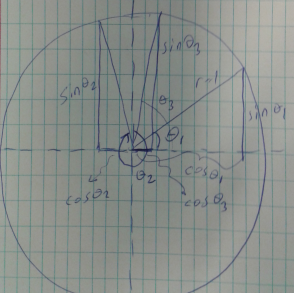
\includegraphics[width=20em]{stat_feat_01.png}

Bu hesabı yapmak için bir yöntem çember, açılar kullanmak. Gün içindeki
zamanı 0 ile 1 arasında kodlarız, sonra bu büyüklüğü $2\pi$ ile çarparız,
bu bize çember üzerindeki bir noktayı verir, yani zamanı açıya çevirmiş
oluruz. Sonra açının $\sin$, $\cos$ değerini hesaplayıp iki rakam elde
ederiz, bu iki sayı bize gün içindeki zamanı temsil eden bir büyüklük
verir.

Bu büyüklükleri birbirleri ile karşılaştırmak daha kolay, üstteki şekilde
$\theta_2$ ve $\theta_3$ birbirine yakın, karşılaştırma yaparken $\sin$
bize dikey eksendeki izdüşümü, $\cos$ yatay eksendeki izdüşümünü verir,
$\theta_2,\theta_3$ için y eksenindeki yansıma birbirine çok yakın. Eksen x
üzerindeki yansıma farklı biri eksi biri artı yönde fakat yine de mutlak
değer bağlamında birbirlerine çok yakınlar. İstediğimiz de bu zaten. 

\begin{minted}[fontsize=\footnotesize]{python}
import scipy.linalg as lin

t1 = 0.12 * 2*np.pi
t2 = 0.97 * 2*np.pi
t3 = 0.03 * 2*np.pi

d1 = (np.cos(t1), np.sin(t1))
d2 = (np.cos(t2), np.sin(t2))
d3 = (np.cos(t3), np.sin(t3))

print ("%f %f" % d1)
print ("%f %f" % d2)
print ("%f %f" % d3)

print u'uzaklık 1-2 =', lin.norm(np.array(d1)-np.array(d2))
print u'uzaklık 2-3 =', lin.norm(np.array(d2)-np.array(d3))
\end{minted}

\begin{verbatim}
0.728969 0.684547
0.982287 -0.187381
0.982287 0.187381
uzaklık 1-2 = 0.907980999479
uzaklık 2-3 = 0.374762629171
\end{verbatim}

Kaynaklar 

[1] Teetor, {\em R Cookbook}

[2] Scikit-Learn Documentation, {\em 4.2. Feature extraction}, \url{http://scikit-learn.org/dev/modules/feature_extraction.html}

[3] Bayramlı, 
    {\em Fonksiyon Gezmek ve Yield}, 
    \url{https://burakbayramli.github.io/dersblog/sk/2011/02/fonksiyon-gezmek-ve-yield.html}

[4] Bayramlı, Istatistik, {\em Lineer Regresyon}



\end{document}



